\section{Introduction}
\paragraph*{}
Skin cancer is categorized into two types: melanoma skin cancer. 
Detection and classification of unknown pigmented skin lesions can result in early diagnosis of the medical problem. Melanoma is the most dangerous kind of skin cancer accounted for an estimated 16,000 deaths each year from 2014 to 2016 in the United Kingdom (Cancer Research UK, 2020). The melanoma tumour caused by melanocytes can result in uncontrolled and abnormal growth which can spread in the human body (Korotkov and Garcia 2012).
The previous research in 2017 has shown that melanoma was the 20th most common disorder with new incidents of 81,00 and 83,00 in males and females in the United Kingdom \citep*{KOROTKOV201269}.
Dermoscopy is a non-invasive method of examining the pigmented skin, which includes microscopic imaging of the surface structure of pigmented skin lesions \citep*{KOROTKOV201269}.
Early diagnosis of pigmented skin lesions is crucial to classify skin disorders to decrease mortality concerning particular skin disorders. Dermoscopy improves the detection of melanoma compared to detection of disease with naked eyes by analysing the pigmented skin lesion. Previous studies have shown that such tumours can result in higher chances of better treatment and cure of disease by removing the tumour \citep*{CELEBI2007362}.
The current diagnosis method of detection involves using ABCD rule which considers the Asymmetry, Border irregularity, Colour irregularities, Darmascopic structures respectively of common pigmented skin lesions \citep*{LOESCHER2013170}.
People working in busy work environments or less mobility can be victims of belated and slow diagnosis of such dangerous skin cancers.
The automated analysis of pigmented skin lesions using artificial neural networks can be beneficial in optical analysis of microscopic images of pigmented skin lesions. 
The primary targeted audience who benefits from the outcome is the people who are working in busy work environments or people with less mobility are best to use cases which can use such an automated system. Booking a prior appointment with medical professionals based on the urgency of detected medical problems can result in the immediate treatment of patients with more critical conditions. The people with less mobility such as older audiences or people with special needs can detect pigmented skin lesions through online systems in an inconvenient manner. Medical institutions can use such technologies to automate the process of pre-health checkups and overcome the problem of shortage of staff members in case of emergency. Such automated systems can also result in faster diagnosis of medical problems compared to a manual analysis by a clinician. 
Furthermore, manufacturing companies which supply the microscopic medical instruments can also use such intelligent models with their products to provide value to customers and medical institutions.


\paragraph{ The research focuses}
 on developing  Convolutional Neural Network for automated optical analysis of pigmented skin lesions.
 
\section{Pigmented Skin Lesions}
1. Melanoma. 
2. Benign keratosis-like lesions.
3. Melanocytic nevi. 
4. Vascular lesions.
\pagebreak
\pagebreak
\section{Bioligical Inspiration for Neural Networks}
The human brain are componsed of millions specialised cell "neurons" which are interconnected to each other which carry electrical and chemical signals from neuron to another to function
There are an estimated 500 trillion connections between neurons in the human nervous system which helps communicate signals \citep*{patterson2017deep}.
The fundamental component of neural networks, which is the perceptron model, is inspired by the single neuron structure.
\subsection*{Structure of Neurons}
\vspace{3mm}
\begin{center}
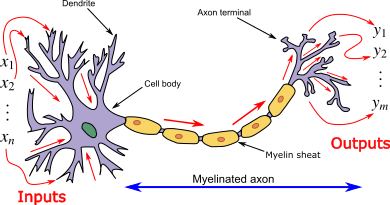
\includegraphics[width=10cm]{Images/neuron.png}
\end{center}

The figure above represents the biological structure of neurons that helps in the communication of electric signals in the nervous system to learn and process information. The biological structure of neurons
includes three major parts dendrites which are responsible for accepting the electrical and chemical signals to the neuron. 
Furthermore, the neuron contains the nucleus which is accountable for the processing input information with the neurons. 
At last, the processed information is passed to another neuron which is interconnected to neurons in the human nervous system through axon terminals
\citep{AGATONOVICKUSTRIN2000717}. 

\subsection{Perceptron Model}
\pagebreak
\section{Artifical Neural Networks}
In this section, you should describe the problem that you set out to solve with the project. An introduction might, for example, begin by stating, "The aim of the work described in this Report was to provide a software tool with which people can arrange meetings." Avoid starting a Report with an irrelevant history of information technology. For example, the following would not be a good introductory sentence, "Since Bill Gates launched Outlook people have been using technology to arrange meetings."
Explain whatever background the reader will need in order to understand the problem. The background might refer to previous work in the academic literature that provides evidence that the problem is a real and significant problem worth solving. The background may identify a community, organisation or set of users that will benefit from your research. Include a clear and detailed statement of the project aims and provide an overview of the structure of the solution.
Explain whatever background the reader will need in order to understand the problem. The background might refer to previous work in the academic literature that provides evidence that the problem is a real and significant problem worth solving. The background may identify a community, organisation or set of users that will benefit from your research. Include a clear and detailed statement of the project aims and provide an overview of the structure of the solution.
CRITICAL! Use the introduction to define any terms or jargon that you will be using throughout the rest of the report.  Why?  Because people define and understand terms differently from one another.  Your definition of ‘cloud computing’ may be different to your supervisor’s definition of ‘cloud computing’.  By stating your definition clearly you can avoid misunderstandings of your work.
Conventionally, the last part of the introduction outlines the remainder of the Report, explaining what comes in each section – keep this brief.
In this section, you should describe the problem that you set out to solve with the project. An introduction might, for example, begin by stating, "The aim of the work described in this Report was to provide a software tool with which people can arrange meetings." Avoid starting a Report with an irrelevant history of information technology. For example, the following would not be a good introductory sentence, "Since Bill Gates launched Outlook people have been using technology to arrange meetings."
Explain whatever background the reader will need in order to understand the problem. The background might refer to previous work in the academic literature that provides evidence that the problem is a real and significant problem worth solving. The background may identify a community, organisation or set of users that will benefit from your research. Include a clear and detailed statement of the project aims and provide an overview of the structure of the solution.
Explain whatever background the reader will need in order to understand the problem. The background might refer to previous work in the academic literature that provides evidence that the problem is a real and significant problem worth solving. The background may identify a community, organisation or set of users that will benefit from your research. Include a clear and detailed statement of the project aims and provide an overview of the structure of the solution.
CRITICAL! Use the introduction to define any terms or jargon that you will be using throughout the rest of the report.  Why?  Because people define and understand terms differently from one another.  Your definition of ‘cloud computing’ may be different to your supervisor’s definition of ‘cloud computing’.  By stating your definition clearly you can avoid misunderstandings of your work.
Conventionally, the last part of the introduction outlines the remainder of the Report, explaining what comes in each section – keep this brief.
\subsection{Deep Neural Networks}
\subsection{Backpropagation}
